\documentclass[11pt, letterpaper]{article}
\usepackage{amsmath, amssymb}
\usepackage{hyperref}
\usepackage{booktabs}
\usepackage{enumitem}
\usepackage{xcolor}
\usepackage{geometry}
\usepackage{fancyhdr}
\usepackage{titlesec}
\usepackage{tcolorbox}
\usepackage{graphicx}
\usepackage{caption}
\usepackage{subcaption}
\usepackage{parskip}
\geometry{margin=1in}

\definecolor{courseblue}{HTML}{002452}
\definecolor{coursegold}{HTML}{FABD0F}
\definecolor{coursered}{HTML}{B90E31}
\definecolor{lightblue}{HTML}{E8EEF7}
\definecolor{lightgold}{HTML}{FEF8E3}

\hypersetup{colorlinks=true,linkcolor=courseblue,urlcolor=coursered}
\tcbuselibrary{skins}
\newtcolorbox{guidancebox}{enhanced,colback=lightblue,colframe=courseblue,
  sharp corners,leftrule=4pt,left=6pt,right=6pt,top=4pt,bottom=4pt}

\pagestyle{fancy}\fancyhf{}
\fancyhead[L]{\small\textcolor{courseblue}{\textbf{CISC 473 --- Deep Learning | Fall 2026}}}
\fancyhead[R]{\small\textcolor{courseblue}{Final Report}}
\fancyfoot[C]{\small\thepage}
\renewcommand{\headrulewidth}{0.4pt}
\titleformat{\section}{\large\bfseries\color{courseblue}}{}{0em}{}[\titlerule]
\titleformat{\subsection}{\normalsize\bfseries\color{courseblue}}{}{0em}{}


\begin{document}

{\centering
  {\Large\textbf{CISC 473: Deep Learning --- Final Report}}\\[0.5em]
  {\large\textit{P02: Zero-Reference Low-Light Image Enhancement for Extremely Dark and Underwater Scenes}}\\[0.4em]
  \textbf{Group Members:}\\
  {Andrew Oh} (Project Lead) \quad
  {Ray Shi} (Research Lead) \quad
  {Abominable Snowman} (Engineering Lead)\\[0.3em]
  \textbf{GitHub:} \url{https://github.com/woong5115/CISC473Project} \quad \textbf{Date:} \today\\[0.4em]
  \rule{\linewidth}{0.4pt}
}

\begin{abstract}
Low-light image enhancement is a prerequisite for reliable computer vision in
settings such as nighttime driving, surveillance, and underwater exploration, yet
supervised enhancers need aligned low-/normal-light image pairs that are costly or
impossible to collect. Zero-DCE and Zero-DCE++ avoid paired data by training a
lightweight network to predict pixel-wise light-enhancement curves with
non-reference losses only. We reproduce both methods on the SICE benchmark and
investigate why our midterm reproduction fell 4--7~dB short of the published PSNR.
A one-factor-at-a-time gap analysis shows that the cause was our evaluation
protocol, not training: scoring outputs against the reference instead of the
low-light input recovers 85--90\% of the gap, and the authors' released
checkpoints reach 15.93 and 16.00~dB under our corrected protocol. We then propose
two training-only losses for Zero-DCE++: a Max-RGB-guided Dynamic Exposure Control
loss that gives shadow regions darker exposure targets, and a Ratio-Locking
Spatial-Color Consistency loss that preserves local RGB proportions. Over three
seeds, ratio-locking alone improves PSNR from $15.00 \pm 0.06$ to
$15.24 \pm 0.04$~dB at no inference cost, with a slight SSIM drop
(0.504 $\to$ 0.493). Dynamic exposure reduces over-saturation
on an underwater example (blown-out pixels: 17.3\% $\to$ 6.9\%) but lowers SICE
PSNR to $13.53 \pm 0.03$~dB, and the full model reaches $13.19 \pm 0.05$~dB. We
trace this drop to a mismatch between darker exposure targets and SICE's
well-exposed references, and discuss what it implies for evaluating zero-reference
enhancement.
\end{abstract}

\section{Introduction}

Low-light images suffer from low visibility, contrast, and strong noise, which
hurts downstream systems for nighttime driving, surveillance, and underwater
exploration, where colour casts and haze are added on top of low light [5]. Most deep enhancers [3, 4, 7] are trained on aligned
low-/normal-light pairs, which are expensive to capture in static scenes and
practically impossible in dynamic ones, so they generalise poorly to domains without
paired data.

Zero-DCE [1] avoids this bottleneck by estimating image-specific curves with a
small network trained only on non-reference losses, and Zero-DCE++ [2] makes it
faster and lighter. Their losses, however, have two blind spots. The exposure loss pulls every region toward the same grey level, so
genuinely dark regions are over-brightened and washed out; and the colour
constancy loss constrains only global channel means, so local colour shifts are
unconstrained. In our midterm experiments, an almost black background with RGB
values of $(16, 4, 18)$ turned visibly purple, and underwater images became hazy
and noisy.

Our midterm reproduction also scored 4--7~dB below the published PSNR. We
therefore ask \emph{why} it fell short (preprocessing, training, or evaluation),
and \emph{whether} the two blind spots can be fixed through the training objective
alone, without paired data or extra inference cost.

In summary, our contributions are:
\begin{itemize}[noitemsep]
  \item We reproduce Zero-DCE and Zero-DCE++ on SICE and, through a
    one-factor-at-a-time gap analysis, show that the 4--7~dB gap in our midterm
    results came from the evaluation protocol: correcting it alone recovers
    85--90\% of the gap, and the remaining 0.4--0.6~dB persists even for the
    authors' own checkpoints.
  \item We propose two training-only losses for Zero-DCE++. Ratio-Locking
    Spatial-Color Consistency improves PSNR by 0.24~dB in every seed, at a small
    SSIM cost and with no added parameters or inference time.
  \item We show that Max-RGB-guided Dynamic Exposure Control reduces
    over-saturation but lowers reference-based PSNR by 1.47~dB, and we analyse this
    as a conflict between darker exposure targets and SICE's well-exposed
    references, together with three failure modes of zero-reference curve
    estimation.
\end{itemize}

\section{Related Work}

\textbf{Supervised and Retinex-Based Low-Light Enhancement.} Early deep learning
approaches to low-light image enhancement relied on supervised training with
paired low- and normal-light images. Inspired by Retinex theory, where an image is
decomposed into reflectance and illumination, often initialized via a Max-RGB prior
as in LIME [8], Retinex-Net [7] learns end-to-end decomposition and illumination
adjustment on paired data. To further improve restoration fidelity, MIRNet [4]
employs multi-scale feature extraction with selective kernel fusion to preserve
spatial detail and colour accuracy, while SNR-Aware [3] uses Signal-to-Noise Ratio
priors to dynamically route noisy, low-SNR regions through transformer blocks and
cleaner regions through convolutions. Although these supervised models achieve
strong reference-based benchmarks on terrestrial datasets, their reliance on
aligned ground-truth pairs and heavier architectures limits their scalability to
dynamic or out-of-domain scenes. Unlike these paired methods, our work operates in
a strictly zero-reference setting and keeps the lightweight real-time footprint of
Zero-DCE++.

\textbf{Unsupervised and Zero-Reference Enhancement.} To eliminate paired training
data, unsupervised methods have explored adversarial and self-calibrated
frameworks. EnlightenGAN [9] trains on unpaired low- and normal-light collections
using global-local discriminators and self-regularized perceptual losses, whereas
SCI [10] introduces a self-calibrated illumination learning cascade that converges
rapidly with minimal compute. Going a step further, Zero-DCE [1] requires neither
paired nor unpaired reference images, instead training a lightweight CNN to predict
pixel-wise light-enhancement curves guided solely by four non-reference losses
(spatial consistency, exposure control, colour constancy, and illumination
smoothness). Zero-DCE++ [2] replaces standard convolutions with depthwise separable
convolutions, shares a single curve map across iterations, and downsamples the
input by $12\times$ for real-time inference. Our work builds directly on the
Zero-DCE++ architecture, but differs by targeting two blind spots in its training
objective: static global exposure targets and global-only colour constancy,
strictly through training-only loss modifications.

\textbf{Underwater Image Enhancement and Domain Transfer.} Underwater imagery
presents distinct physical degradations beyond low illumination, notably
wavelength-dependent light absorption (where red light attenuates fastest) and
particulate backscattering haze. Li et al.\ [5] introduced the Underwater Image
Enhancement Benchmark (UIEB) alongside Water-Net, a gated fusion CNN trained on
paired underwater references. Subsequent methods have emphasized either real-time
efficiency, such as FUnIE-GAN [6] using a conditional GAN for robotic visual
perception, or physics-guided colour restoration, such as Ancuti et al.\ [11], which
explicitly compensates the attenuated red channel prior to white-balancing and
fusion. While effective, these approaches rely on paired underwater supervision or
explicit underwater physical models. Our work bridges these literatures by
evaluating zero-reference curve estimation directly on underwater scenes and
diagnosing where training-only exposure and colour-ratio constraints succeed versus
where physical wavelength loss limits monotonic curve enhancers.
Table~\ref{tab:related} in the appendix summarises these methods.

\section{Method}

\subsection{Problem Formulation}

Given a low-light image $I \in [0,1]^{H \times W \times 3}$, a network
$f_\theta$ predicts per-pixel curve parameter maps $\mathcal{A} = f_\theta(I)$,
$A_n \in [-1,1]^{H \times W \times 3}$, and the enhanced image is
$Y = \mathcal{E}(I; \mathcal{A})$. No reference image is available during
training, so $\theta$ minimises a sum of non-reference losses
$\mathcal{L}(I, Y, \mathcal{A})$ over unpaired low-light images.

\subsection{Model Architecture}

The enhancement operator is the light-enhancement curve of Zero-DCE [1],
\begin{equation}
  LE_n(x) = LE_{n-1}(x) + A_n(x)\, LE_{n-1}(x)\bigl(1 - LE_{n-1}(x)\bigr),
  \qquad LE_0 = I, \quad Y = LE_N,
  \label{eq:curve}
\end{equation}
applied per colour channel with $N = 8$ iterations; it is monotonic, keeps outputs
in $[0,1]$, and is differentiable. We use the Zero-DCE++ DCE-Net [2]
(Fig.~\ref{fig:arch}): seven depthwise separable convolution layers with skip
concatenations (32 channels, ReLU), and a Tanh output giving one curve map shared
across all iterations. At test time the curve map is estimated on an input
downsampled by $s = 12$ and upsampled back. Our modifications do not change the
architecture.

\begin{figure}[h]
  \centering
  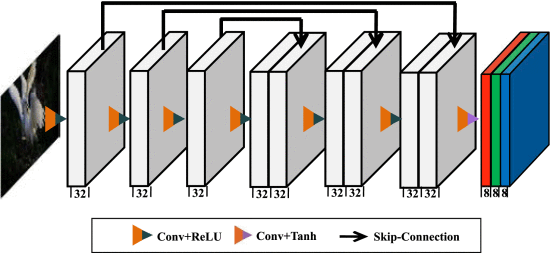
\includegraphics[width=0.42\linewidth]{images/dce-net.png}
  \caption{DCE-Net. A low-light image is mapped to per-pixel curve parameter maps,
  which are applied iteratively by the LE curve of Eq.~\eqref{eq:curve}. Zero-DCE++
  replaces each convolution with a depthwise separable convolution and shares one
  curve map across iterations.}
  \label{fig:arch}
\end{figure}

\subsection{Training Objective}

The baseline objective of Zero-DCE/Zero-DCE++ combines four non-reference losses.
Let $Y_k$ and $I_k$ be the mean intensity (over channels) of local region $k$ in the
enhanced and input images, and let $\Omega(k)$ be its four neighbours.

\emph{Spatial consistency} preserves local contrast between neighbouring
$4\times4$ regions:
\begin{equation}
  \mathcal{L}_{spa} = \frac{1}{K}\sum_{k=1}^{K}\sum_{j\in\Omega(k)}
  \bigl(|Y_k - Y_j| - |I_k - I_j|\bigr)^2 .
\end{equation}
\emph{Exposure control} pulls the mean of each non-overlapping $16\times16$ region
toward a fixed well-exposedness level $E$ (0.6 in [1]):
\begin{equation}
  \mathcal{L}_{exp} = \frac{1}{M}\sum_{k=1}^{M} |Y_k - E| .
  \label{eq:exp}
\end{equation}
\emph{Colour constancy} applies a grey-world prior to the global channel means
$J^p$ of $Y$:
\begin{equation}
  \mathcal{L}_{col} = \sum_{(p,q)\in\varepsilon} (J^p - J^q)^2,
  \qquad \varepsilon = \{(R,G),(R,B),(G,B)\}.
  \label{eq:col}
\end{equation}
\emph{Illumination smoothness} keeps the curve maps spatially smooth:
\begin{equation}
  \mathcal{L}_{tv_{\mathcal{A}}} = \frac{1}{N}\sum_{n=1}^{N}\sum_{c\in\{R,G,B\}}
  \bigl(|\nabla_x A_n^c| + |\nabla_y A_n^c|\bigr)^2 .
\end{equation}
The full objective used in our experiments is
\begin{equation}
  \mathcal{L} = \mathcal{L}_{spa} + W_{exp}\,\mathcal{L}_{exp}^{(\cdot)}
  + W_{col}\,\mathcal{L}_{col} + W_{tv}\,\mathcal{L}_{tv_{\mathcal{A}}}
  + W_{rl}\,\mathcal{L}_{rl},
  \label{eq:loss}
\end{equation}
where $\mathcal{L}_{exp}^{(\cdot)}$ is either the fixed-target loss of
Eq.~\eqref{eq:exp} (baseline) or our dynamic version
$\mathcal{L}_{exp}^{dyn}$ (Sec.~\ref{sec:mod}), and $W_{rl} = 0$ for the baseline.
We use the weights from our released training script: $W_{exp} = 10$,
$W_{col} = 5$, $W_{tv} = 1600$ (200 for Zero-DCE), and $W_{rl} = 50$. As in the
released code, the exposure error is squared rather than taken in absolute value.

\subsection{Proposed Modification}
\label{sec:mod}

\textbf{Dynamic Exposure Control (Max-RGB guided).}
\emph{Hypothesis:} washed-out results come from Eq.~\eqref{eq:exp} asking
\emph{every} region, including true shadows, to reach the same level $E$; darker
targets for shadows should preserve depth and reduce noise amplification. We
estimate illumination with the Max-RGB prior used in Retinex methods [7, 8]:
\begin{equation}
  L(x) = \max_{c\in\{R,G,B\}} I^c(x), \qquad
  \tilde{L}_k = \frac{\bar{L}_k - \min_j \bar{L}_j}{\max_j \bar{L}_j - \min_j \bar{L}_j + \epsilon},
\end{equation}
where $\bar{L}_k$ is the mean of $L$ over region $k$, so $\tilde{L}_k\in[0,1]$ ranks
the region's brightness within the image. Each region gets its own target
\begin{equation}
  E_k = E_{\min} + (E_{\max} - E_{\min})\,\tilde{L}_k, \qquad
  \mathcal{L}_{exp}^{dyn} = \frac{1}{M}\sum_{k=1}^{M} (Y_k - E_k)^2 ,
\end{equation}
with $E_{\min} = 0.4$ and $E_{\max} = 0.7$, so the darkest regions are asked to
reach 0.4 instead of the fixed 0.6. $E_k$ is computed from the input and treated
as a constant; the error is squared as in the baseline, so only the target changes.

\textbf{Ratio-Locking Spatial-Color Consistency.}
\emph{Hypothesis:} Eq.~\eqref{eq:col} constrains only global channel means, so
the per-channel curve can create local tints that average out. We lock the
\emph{chromaticity} of each $4\times4$ region to that of the input:
\begin{equation}
  \rho_k^c(Z) = \frac{\bar{Z}_k^c + \epsilon}{\sum_{c'} \bar{Z}_k^{c'} + 3\epsilon},
  \qquad
  \mathcal{L}_{rl} = \frac{1}{K}\sum_{k=1}^{K}\sum_{c\in\{R,G,B\}}
  \bigl(\rho_k^c(Y) - \rho_k^c(I)\bigr)^2 ,
\end{equation}
where $\bar{Z}_k^c$ is the mean of channel $c$ of $Z$ over region $k$. The loss is
zero when all channels of a region are brightened by the same factor, so it permits
brightening but penalises curve-induced colour shifts; region averaging makes it
robust to per-pixel noise. It preserves the \emph{input's} colour balance and so
cannot remove an existing cast (Sec.~\ref{sec:failure}). We use
$\epsilon = 10^{-3}$ and an untuned $W_{rl} = 50$. Neither loss adds parameters or
inference cost.

\section{Experiments}

\subsection{Experimental Setup}

\begin{tabular}{ll}
\toprule
\textbf{Setting} & \textbf{Value} \\
\midrule
Dataset(s) & SICE [12] Part~1 (3{,}021 train, references unused) / Part~2 (767 test) \\
Metrics & PSNR, SSIM against the SICE reference; inference time \\
Optimiser & Adam, weight decay $10^{-4}$, gradient-norm clip 0.1 \\
Learning rate & $10^{-4}$ (constant) \\
Batch size & 8, training images resized to $256\times256$ \\
Training duration & 30 epochs, mixed precision (FP16 forward, FP32 losses) \\
Seeds & 42, 123, 999 \\
Hardware & Google Colab, NVIDIA T4 GPU \\
\bottomrule
\end{tabular}

\textbf{Data.} Following [1], we keep the darkest three (four) images of each
7-image (9-image) SICE Part~2 sequence; for the 19 sequences of length 5, 6, or 8,
which the paper does not cover, keeping the darkest two or three images yields
exactly the 767 test images of [1]. Test images and references are resized to
$1200\times900$ (Lanczos) and stored losslessly.

\textbf{Compute budget.} At the released setting ($512\times512$, 100 epochs),
Zero-DCE++ took 78~s per epoch on a T4, i.e.\ about 26~GPU-hours for our 12 runs,
beyond the free Colab quota. All retrained models, baseline and proposed alike, are
therefore trained at $256\times256$ (the released Zero-DCE resolution) for 30
epochs with mixed precision, about 10~minutes per run. Comparisons between our runs
are fair; absolute scores are about 1~dB below fully trained models
(Sec.~\ref{sec:gap}). Zero-DCE was evaluated only through checkpoints. Each
configuration is trained with three seeds, and we report the mean $\pm$ std of the
per-seed test averages.

\subsection{Main Results}

\begin{table}[h]
\centering
\begin{tabular}{lcc}
\toprule
\textbf{Method} & \textbf{PSNR (dB)} $\uparrow$ & \textbf{SSIM} $\uparrow$ \\
\midrule
Zero-DCE (Pub.\ [1]) & 16.57 & 0.59 \\
Zero-DCE++ (Pub.\ [2]) & 16.42 & 0.58 \\
Zero-DCE, released checkpoint (our eval.) & 15.93 & 0.497 \\
Zero-DCE++, released checkpoint (our eval.) & \textbf{16.00} & \textbf{0.508} \\
\midrule
Zero-DCE++, our retraining (baseline) & 15.00 $\pm$ 0.06 & \textbf{0.504 $\pm$ $<$0.001} \\
Ours: + Ratio-Lock & \textbf{15.24 $\pm$ 0.04} & 0.493 $\pm$ 0.002 \\
Ours: full (+ Dyn.\ Exp.\ + Ratio-Lock) & 13.19 $\pm$ 0.05 & 0.420 $\pm$ 0.003 \\
\bottomrule
\end{tabular}
\caption{Results on SICE Part~2 (767 images). Rows below the line are trained by us
under the same budget (Sec.~4.1) and report mean $\pm$ std over 3 seeds; bold marks
the best value in each block. Published SSIM values are not directly comparable to
ours (Sec.~\ref{sec:gap}).}
\label{tab:main}
\end{table}

\textbf{Reproduction.} Under the corrected protocol, the released checkpoints
reach 15.93~dB (Zero-DCE) and 16.00~dB (Zero-DCE++), within 0.64 and 0.42~dB of the
published values (Sec.~\ref{sec:gap}). Our reduced-budget Zero-DCE++ baseline
reaches $15.00 \pm 0.06$~dB. Zero-DCE++ processes a $1200\times900$ image in
12.8~ms versus 64.4~ms for Zero-DCE on the T4 (5.0$\times$ faster) while scoring
0.07~dB higher, consistent with [2].

\textbf{Proposed losses.} Ratio-locking raises PSNR from $15.00 \pm 0.06$ to
$15.24 \pm 0.04$~dB; the gain is small but holds for every seed (+0.30, +0.12,
and +0.30~dB for seeds 42, 123, 999). SSIM, however, falls slightly in every seed,
from 0.504 to 0.493, so ratio-locking trades a little structural similarity for
intensity fidelity. The full model, however,
scores $13.19 \pm 0.05$~dB, 1.81~dB \emph{below} the baseline, with SSIM falling
from 0.504 to 0.420. Section~\ref{sec:abl} traces this to the dynamic exposure
loss, so our hypothesis for the full model is not confirmed under reference-based
metrics.

\subsection{Reproduction Gap Analysis}
\label{sec:gap}

Following the TA's suggestion, we split every difference between our midterm
pipeline and the published one into evaluation, preprocessing, and training, and
changed one factor at a time (Table~\ref{tab:gap}). Auditing the midterm notebook
showed that PSNR and SSIM had been computed against the \emph{low-light input}
rather than the SICE reference, that test images were saved as lossy JPEG, and
that the ``three seeds'' re-scored identical outputs because training was commented
out. Moreover, the midterm Zero-DCE checkpoint is byte-for-byte identical (same MD5
hash) to the authors' released file, so its gap could not have come from training.

\begin{table}[h]
\centering
\small\setlength{\tabcolsep}{4pt}
\begin{tabular}{llcc}
\toprule
\textbf{ID} & \textbf{Change} & \textbf{Zero-DCE} & \textbf{Zero-DCE++} \\
\midrule
M  & Midterm pipeline (ref.\ = input, JPEG) & 12.22$^\dagger$ & 9.50$^\dagger$ \\
M$'$ & Midterm checkpoints, lossless PNG (ref.\ = input) & 12.35 & 9.24 \\
E1 & Midterm checkpoints, ref.\ = SICE reference & \textbf{15.93} & \textbf{15.68} \\
E3 & Authors' released checkpoints, E1 protocol & 15.93$^\ddagger$ & 16.00 \\
E2 & Retrained, reduced budget (3 seeds) & -- & 15.00 $\pm$ 0.06 \\
P1 & E2 + bilinear test resizing & -- & 15.12 $\pm$ 0.06 \\
P2 & P1 + 7/9-image sequences only (727 images) & -- & 15.06 $\pm$ 0.06 \\
\midrule
-- & Published [1, 2] & 16.57 & 16.42 \\
\bottomrule
\end{tabular}
\caption{Reproduction gap analysis on SICE Part~2 (PSNR in dB).
$^\dagger$Midterm values measured against the low-light input.
$^\ddagger$Identical to E1 because the midterm Zero-DCE checkpoint is the authors'
file. SSIM values are given in the appendix.}
\label{tab:gap}
\end{table}

\textbf{Evaluation explains most of the gap.} Re-scoring the \emph{same}
checkpoints against the reference (M$'$ $\to$ E1) raises PSNR from 12.35 to
15.93~dB for Zero-DCE (+3.58~dB) and from 9.24 to 15.68~dB for Zero-DCE++
(+6.44~dB), closing 85\% and 90\% of the gaps, and makes Zero-DCE++ within 0.25~dB of
Zero-DCE, as [2] reports, rather than 3~dB worse. JPEG compression mattered little
(M vs.\ M$'$: $+0.13$ and $-0.26$~dB).

\textbf{Preprocessing matters little; training budget matters more.} The two
unspecified preprocessing choices change PSNR by at most 0.12~dB (P1, P2), so they
cannot explain the 0.42--0.64~dB residual of the released checkpoints, which must
come from unreported test-preparation or metric details. Our own training costs
about 1~dB: 0.32~dB for the midterm checkpoint (E1 vs.\ E3) and 1.0~dB for the
reduced-budget retraining (E2 vs.\ E3). The SSIM gap (0.50 vs.\ 0.58--0.59) also
persists for the released checkpoints, so we compare SSIM only between our runs.

\subsection{Ablation Study}
\label{sec:abl}

\begin{table}[h]
\centering
\begin{tabular}{lcccc}
\toprule
\textbf{Configuration} & \textbf{Dyn.\ Exp.} & \textbf{Ratio-Lock} & \textbf{PSNR} $\uparrow$ & \textbf{SSIM} $\uparrow$ \\
\midrule
Full model (ours) & \checkmark & \checkmark & 13.19 $\pm$ 0.05 & 0.420 $\pm$ 0.003 \\
w/o Ratio-Lock & \checkmark & $\times$ & 13.53 $\pm$ 0.03 & 0.441 $\pm$ 0.002 \\
w/o Dyn.\ Exp. & $\times$ & \checkmark & \textbf{15.24 $\pm$ 0.04} & 0.493 $\pm$ 0.002 \\
Baseline (Zero-DCE++) & $\times$ & $\times$ & 15.00 $\pm$ 0.06 & \textbf{0.504 $\pm$ $<$0.001} \\
\bottomrule
\end{tabular}
\caption{Ablation on SICE Part~2. Each row is mean $\pm$ std over 3 seeds under the
same training budget.}
\label{tab:ablation}
\end{table}

Adding one component at a time to the baseline (Table~\ref{tab:ablation})
separates the two losses. Ratio-locking alone gives $+0.24$~dB PSNR but $-0.011$
SSIM; dynamic exposure alone gives $-1.47$~dB, the opposite of what we expected. The effects are not
additive: their sum predicts $-1.23$~dB, but the full model loses 1.81~dB, so
ratio-locking stops helping once exposure targets are lowered, plausibly because
the input's channel proportions it preserves are least reliable in dark,
colour-biased regions.

\textbf{Why does dynamic exposure lower PSNR?} The loss does what it was designed
to do: on the underwater example of Fig.~\ref{fig:qual}, blown-out pixels (mean
intensity $>0.9$) fall from 17.3\% to 6.9\%, mean brightness from 0.65 to 0.51, and
contrast (pixel std) rises from 0.230 to 0.250. But SICE references are bright, and
PSNR compares absolute intensities, so deliberately darker shadows are penalised.
Whether trading fidelity to SICE's exposure for less saturation is desirable cannot
be decided by PSNR; it needs a perceptual study or no-reference metric.

\subsection{Qualitative Analysis}

\begin{figure}[h]
  \centering
  \begin{subfigure}{0.24\linewidth}
    
\includegraphics[width=\linewidth]{images/trooper-before.jpg}
    \caption{Dark input}
  \end{subfigure}\hfill
  \begin{subfigure}{0.24\linewidth}
    
\includegraphics[width=\linewidth]{images/trooper-after.jpg}
    \caption{Zero-DCE (released)}
  \end{subfigure}\hfill
  \begin{subfigure}{0.24\linewidth}
    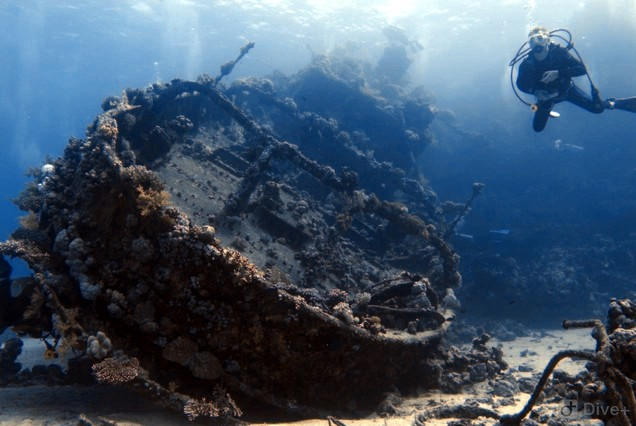
\includegraphics[width=\linewidth]{images/q392_input.jpg}
    \caption{UIEB input}
  \end{subfigure}\hfill
  \begin{subfigure}{0.24\linewidth}
    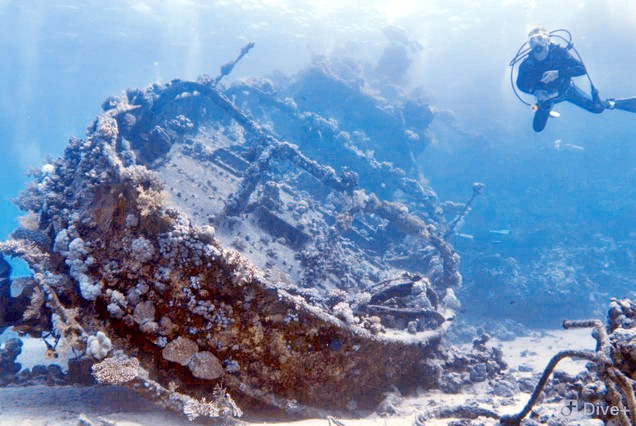
\includegraphics[width=\linewidth]{images/q392_authors_dcepp.jpg}
    \caption{Zero-DCE++ (released)}
  \end{subfigure}\\[0.4em]
  \begin{subfigure}{0.24\linewidth}
    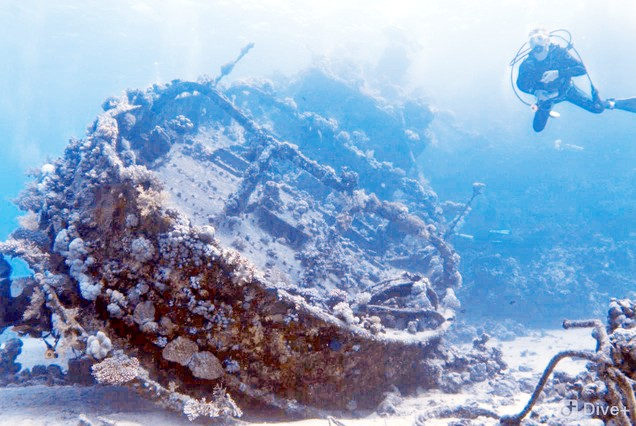
\includegraphics[width=\linewidth]{images/q392_base.jpg}
    \caption{Our baseline}
  \end{subfigure}\hfill
  \begin{subfigure}{0.24\linewidth}
    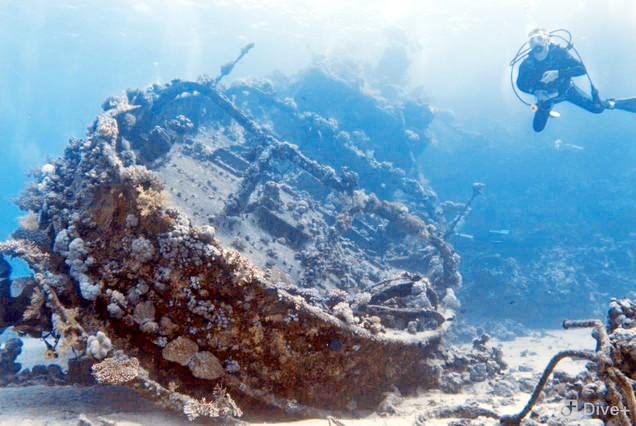
\includegraphics[width=\linewidth]{images/q392_rl.jpg}
    \caption{+ Ratio-Lock}
  \end{subfigure}\hfill
  \begin{subfigure}{0.24\linewidth}
    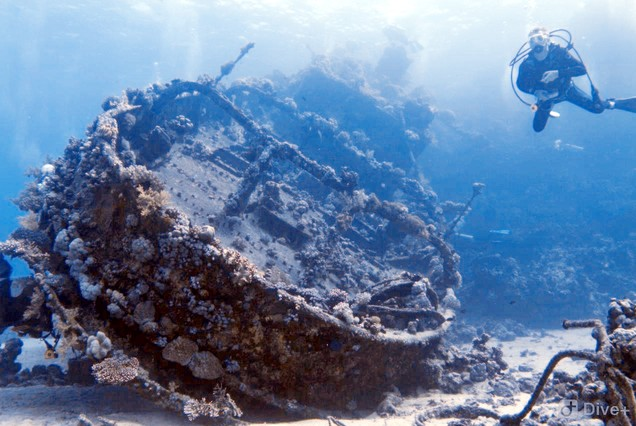
\includegraphics[width=\linewidth]{images/q392_dyn.jpg}
    \caption{+ Dyn.\ Exp.}
  \end{subfigure}\hfill
  \begin{subfigure}{0.24\linewidth}
    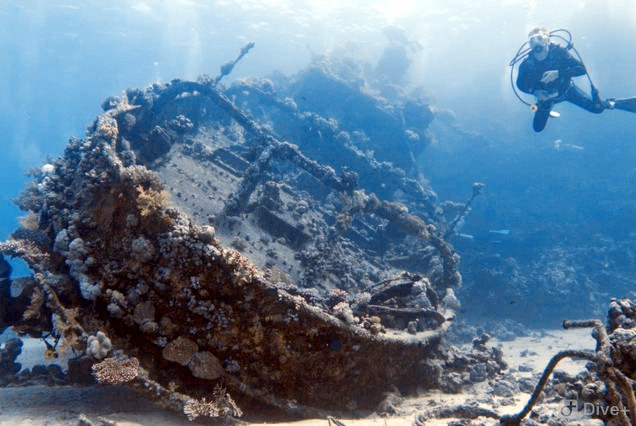
\includegraphics[width=\linewidth]{images/q392_full.jpg}
    \caption{Full model}
  \end{subfigure}
  \caption{(a)--(b): purple tint of the released Zero-DCE on an extremely dark image.
  (c)--(h): an underwater UIEB image (not used for training) enhanced by the released
  Zero-DCE++ and by our models (seed 42).}
  \label{fig:qual}
\end{figure}

In Fig.~\ref{fig:qual}(b) the almost black background becomes flat magenta. Our
reduced-budget baseline (e) turns the water milky and saturates the top; ratio-locking
(f) looks similar; dynamic exposure (g, h) keeps deep water and the shadowed hull
darker, with more depth and contrast, closer to the released model (d), while all
models keep the blue cast.

\subsection{Failure Analysis}
\label{sec:failure}

\paragraph{Failure type 1:} Input-inherited colour casts in extremely dark regions ---
In Fig.~\ref{fig:qual}(a) a background pixel is about $(16, 4, 18)$, already
purple. For small $I$, Eq.~\eqref{eq:curve} acts like a per-channel gain $I(1+A)$,
so the ratios survive and the cast becomes visible once brightened (b). The global
colour loss is dominated by the bright foreground, and ratio-locking preserves input
proportions by design. \emph{Mitigation:}
apply a grey-world constraint locally, weighted toward dark regions.

\paragraph{Failure type 2:} Noise amplification --- The curve multiplies signal and noise
alike, and no loss measures noise (the smoothness loss acts on the curve map, not
the output). Lower exposure targets reduce shadow gain and hence noise, but at the
PSNR cost of Sec.~\ref{sec:abl}.
\emph{Mitigation:} an edge-preserving denoiser on dark regions, or an SNR-weighted
exposure loss as in [3].

\paragraph{Failure type 3:} Underwater colour cannot be restored by brightening ---
Water absorbs red light first (in Fig.~\ref{fig:qual}(c) mean red is 0.61 times
blue). A monotonic per-channel curve can scale but not create missing red signal, so
every model keeps the blue cast (in (h) blue is still 1.5 times red), and the
exposure loss brightens backscatter haze instead of removing it.
\emph{Mitigation:} physics-based red-channel compensation [11] before curve
estimation.

\paragraph{Failure type 4:} Proposed loss versus evaluation target --- Dynamic
exposure fails numerically on SICE although it reduces saturation, because its
darker targets disagree with the bright references (Sec.~\ref{sec:abl}): a
zero-reference loss may choose any exposure, but a reference benchmark rewards one. \emph{Mitigation:} tune $E_{\min}$
on a validation split and add perceptual metrics.

\section{Discussion}

Our reproduction gap was an evaluation error, not a modelling problem: evaluation
pipelines should be validated on released checkpoints \emph{before} drawing
conclusions about training. Ratio-locking gives a small, consistent PSNR gain at a
slight SSIM cost, while dynamic exposure behaves as intended but is penalised
because SICE defines ``correct'' exposure as bright, a tension for zero-reference
methods judged on reference benchmarks.

\subsection{Limitations}

Our models use a reduced training budget and untuned $E_{\min}$, $E_{\max}$, $W_{rl}$;
we report reference-based metrics on one benchmark, our underwater evidence is
qualitative, we ran no user study, and a 0.4--0.6~dB residual remains unexplained.

\section{Conclusion}

Our midterm reproduction gap was almost entirely an evaluation error; the released
checkpoints come within 0.6~dB of the published results. Ratio-locking improves
Zero-DCE++ by 0.24~dB PSNR at a small SSIM cost, while dynamic exposure reduces
over-saturation at a 1.5~dB PSNR cost; tuning its range and adding perceptual
evaluation is the natural next step.

\section{AI Tool Disclosure}

We used Claude (Anthropic, claude.ai) to help draft and edit sections of this report
from our proposal, midterm report, code, and experiment logs; to write the Colab
notebook that runs the experiments and computes the metrics; and to suggest the
formal notation for our proposed losses. We also used Google Gemini to assist with
Related Work synthesis, reference formatting and verification, and document
organization. All experiments were run by us, all numbers in this report come from
those runs, and we verified all AI-generated text, citations, and code against our
results and the original primary papers.

\section{Contribution Declaration}

\begin{tabular}{lcc}
\toprule
\textbf{Member} & \textbf{Contributions} & \textbf{\%} \\
\midrule
{Andrew Oh} & Project management, experiments, report writing & 33.3\% \\
{Ray Shi} & Literature review, metrics evaluation, ablation studies & 33.3\% \\
{Abominable Snowman} & Model coding, baseline reproduction, GitHub, README & 33.3\% \\
\bottomrule
\end{tabular}

\section{References}

{\sloppy
\begin{enumerate}[label={[\arabic*]},leftmargin=*]
  \item Guo, C., Li, C., Guo, J., Loy, C. C., Hou, J., Kwong, S., \& Cong, R., 2020.
    ``Zero-Reference Deep Curve Estimation for Low-Light Image Enhancement.''
    \textit{CVPR}. arXiv:2001.06826.
  \item Li, C., Guo, C., \& Loy, C. C., 2021. ``Learning to Enhance Low-Light Image
    via Zero-Reference Deep Curve Estimation.'' \textit{IEEE TPAMI}. arXiv:2103.00860.
  \item Xu, X., Wang, R., Fu, C.-W., \& Jia, J., 2022. ``SNR-Aware Low-Light Image
    Enhancement.'' \textit{CVPR}. DOI:10.1109/CVPR52688.2022.01719.
  \item Zamir, S. W., Arora, A., Khan, S., Hayat, M., Khan, F. S., Yang, M.-H., \&
    Shao, L., 2020. ``Learning Enriched Features for Real Image Restoration and
    Enhancement.'' \textit{ECCV}. arXiv:2003.06792.
  \item Li, C., Guo, C., Ren, W., Cong, R., Hou, J., Kwong, S., \& Tao, D., 2019.
    ``An Underwater Image Enhancement Benchmark Dataset and Beyond.''
    \textit{IEEE TIP}. arXiv:1901.05495.
  \item Islam, M. J., Xia, Y., \& Sattar, J., 2020. ``Fast Underwater Image
    Enhancement for Improved Visual Perception.'' \textit{IEEE RA-L}.
    arXiv:1903.09766.
  \item Wei, C., Wang, W., Yang, W., \& Liu, J., 2018. ``Deep Retinex Decomposition
    for Low-Light Enhancement.'' \textit{BMVC}. arXiv:1808.04560.
  \item Guo, X., Li, Y., \& Ling, H., 2017. ``LIME: Low-Light Image Enhancement via
    Illumination Map Estimation.'' \textit{IEEE TIP}. DOI:10.1109/TIP.2016.2639450.
  \item Jiang, Y., Gong, X., Liu, D., Cheng, Y., Fang, C., Shen, X., Yang, J., Zhou,
    P., \& Wang, Z., 2021. ``EnlightenGAN: Deep Light Enhancement Without Paired
    Supervision.'' \textit{IEEE TIP}. arXiv:1906.06972.
  \item Ma, L., Ma, T., Liu, R., Fan, X., \& Luo, Z., 2022. ``Toward Fast, Flexible,
    and Robust Low-Light Image Enhancement.'' \textit{CVPR}. arXiv:2204.10137.
  \item Ancuti, C. O., Ancuti, C., De Vleeschouwer, C., \& Bekaert, P., 2018.
    ``Color Balance and Fusion for Underwater Image Enhancement.''
    \textit{IEEE TIP}. DOI:10.1109/TIP.2017.2759252.
  \item Cai, J., Gu, S., \& Zhang, L., 2018. ``Learning a Deep Single Image Contrast
    Enhancer from Multi-Exposure Images.'' \textit{IEEE TIP}.
\end{enumerate}
}

\appendix

\section{Appendix: Additional Results}

\textbf{Gap analysis, SSIM.} M$'$: 0.531 (Zero-DCE) / 0.444 (Zero-DCE++);
E1: 0.497 / 0.511; E3: 0.497 / 0.508; E2: 0.504 $\pm$ $<$0.001; P1: 0.529 $\pm$ 0.001;
P2: 0.525 $\pm$ 0.001; published: 0.59 / 0.58. Bilinear resizing raises SSIM by
0.025, more than it raises PSNR, consistent with its smoothing effect. The midterm
report listed an SSIM of 0.46 for Zero-DCE, while the corresponding notebook output
was 0.53; both were measured against the input and are superseded here.

\textbf{Implementation notes.} The released Zero-DCE++ training script squares the
exposure error instead of taking its absolute value and uses loss weights
$W_{exp}=10$, $W_{col}=5$, $W_{tv}=1600$; we keep these choices for all
configurations. Inference uses the downsampling factor $s=12$, so test images are
cropped to $1200\times900$ (already a multiple of 12). Our SSIM implementation
reproduces \texttt{skimage.metrics.structural\_similarity} (7$\times$7 uniform
window, colour, data range 255) exactly; we verified this numerically.

\textbf{Brightness statistics for Fig.~\ref{fig:qual}(c)--(h)} (mean intensity /
share of pixels with mean $>0.9$ / std): input 0.333 / 2.8\% / 0.256; released
Zero-DCE++ 0.576 / 6.4\% / 0.218; our baseline 0.650 / 17.3\% / 0.230; + Ratio-Lock
0.582 / 10.5\% / 0.238; + Dyn.\ Exp.\ 0.511 / 6.9\% / 0.250; full 0.475 / 5.9\% / 0.252.

\begin{table}[h]
\centering
\small
\begin{tabular}{p{2.4cm}p{0.9cm}p{4.6cm}p{5.2cm}}
\toprule
\textbf{Method} & \textbf{Year} & \textbf{Key Idea} & \textbf{Relation to Our Work} \\
\midrule
Zero-DCE [1] & 2020 & Image-specific LE curve estimation trained with four non-reference losses. & Core zero-reference framework and secondary baseline. \\
Zero-DCE++ [2] & 2021 & Depthwise separable convolutions, shared curve map, and $12\times$ downsampling. & Primary architectural baseline extended by our training-only losses. \\
SNR-Aware [3] & 2022 & Signal-to-Noise Ratio priors routing noisy regions to transformers. & Supervised noise-aware contrast; motivates our noise mitigation analysis. \\
MIRNet [4] & 2020 & Multi-scale feature extraction and selective kernel fusion on paired data. & Paired restoration benchmark contrasted against zero-reference training. \\
Water-Net / UIEB [5] & 2019 & Gated fusion CNN and the 950-image UIEB underwater benchmark. & Provides our out-of-domain underwater evaluation image and context. \\
FUnIE-GAN [6] & 2020 & Real-time conditional GAN for underwater visual perception. & Underwater real-time baseline contrasted against curve estimation. \\
Retinex-Net [7] & 2018 & Paired deep Retinex decomposition into reflectance and illumination. & Paired Retinex enhancer; motivates our Max-RGB illumination prior. \\
LIME [8] & 2017 & Classical Max-RGB illumination map estimation with structural refinement. & Direct inspiration for our local Max-RGB dynamic exposure target. \\
EnlightenGAN [9] & 2021 & Unpaired GAN-based enhancement with global-local discriminators. & Unsupervised contrast requiring unpaired normal-light target sets. \\
SCI [10] & 2022 & Self-calibrated illumination cascade for fast unsupervised LLIE. & Lightweight unsupervised alternative to curve estimation. \\
Ancuti et al.\ [11] & 2018 & Physics-based red-channel compensation and multi-scale fusion. & Motivates our proposed mitigation for underwater red-channel attenuation. \\
\bottomrule
\end{tabular}
\caption{Summary of related work.}
\label{tab:related}
\end{table}

\section{Appendix: Reproducibility Checklist}

All items are satisfied by the repository linked in the header.

\begin{itemize}[noitemsep]
  \item[$\boxtimes$] \texttt{README.md} explains how to reproduce all main results with one command.
  \item[$\boxtimes$] \texttt{requirements.txt} or \texttt{environment.yml} lists all dependencies with versions.
  \item[$\boxtimes$] All random seeds are fixed and documented.
  \item[$\boxtimes$] All results are mean $\pm$ std over $\geq$3 independent runs.
  \item[$\boxtimes$] GitHub repository is public and the link is in the report header.
  \item[$\boxtimes$] No hard-coded absolute paths in any script.
  \item[$\boxtimes$] All datasets are downloaded programmatically or clearly documented.
  \item[$\boxtimes$] Model checkpoints or inference instructions are included (if model is too large, document how to retrain from scratch).
\end{itemize}

\end{document}
